\documentclass[../main.tex]{subfiles}

\begin{document}

The endpoint serves for creation of internal SCM repository – such repository is present in the internal Red Hat GitLab instance. In addition, the created repository is under PNC workspace, which is important in order to guarantee that Reqour has write permissions into a repository.

In addition, repositories can be further nested under organization (which is almost exclusively the case, i.e., only very few repositories are directly under PNC workspace). The complete hierarchy is depicted in Figure \ref{fig:gitlab-hierarchy}.

\begin{figure}
  \begin{center}
    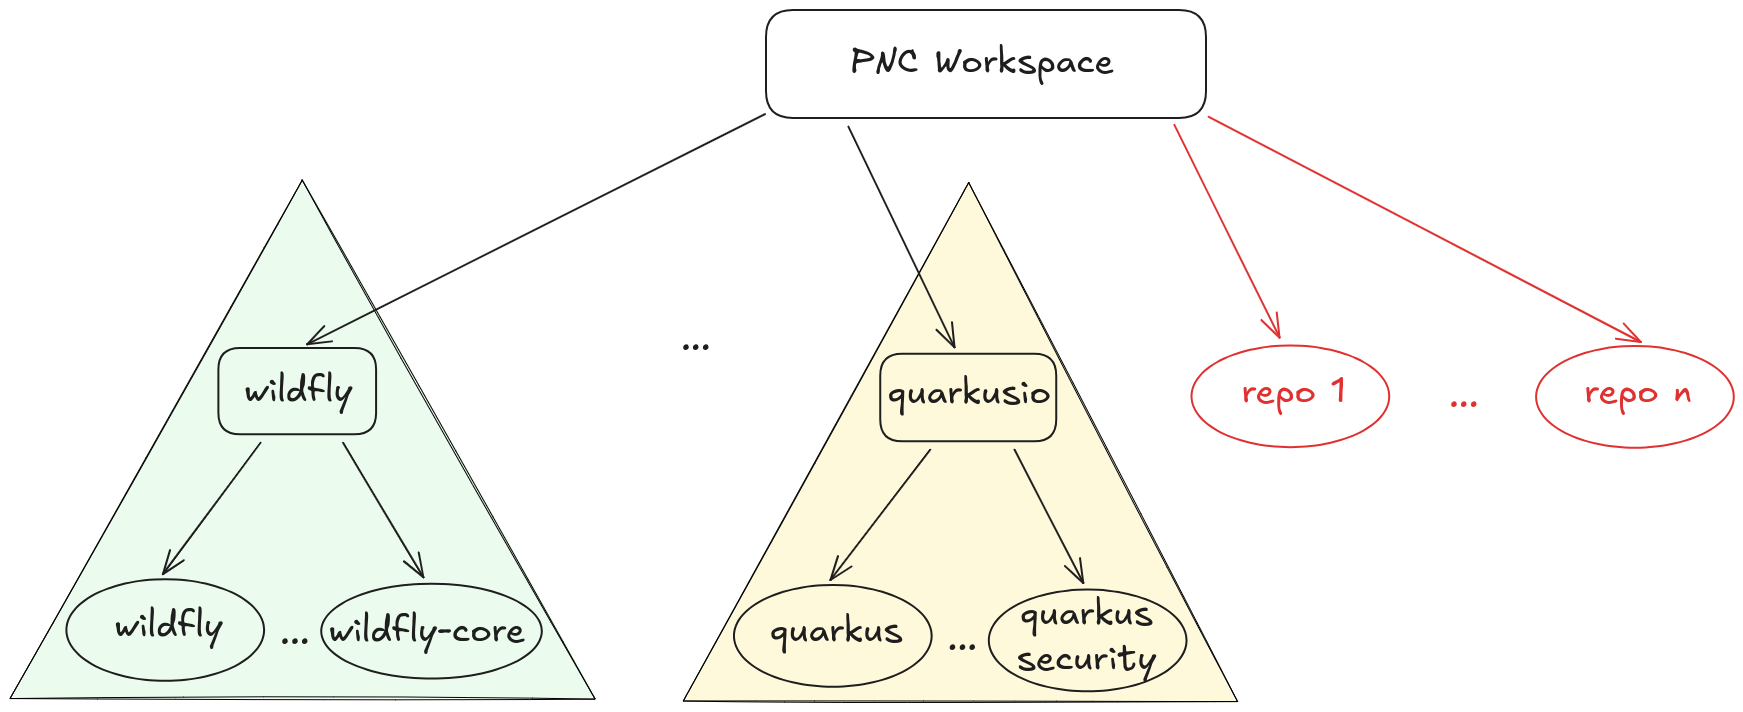
\includegraphics[width=\textwidth]{images/gitlab-hierarchy.png}
  \end{center}
  \caption{Hierarchy under PNC workspace at GitLab}
  \label{fig:gitlab-hierarchy}
\end{figure}

\end{document}
